\documentclass[12pt,aspectratio=169,svgnames]{beamer}

\usepackage{modules/cgs}

\begin{document} \maketitle

\begin{frame}{Содержание}
	\tableofcontents
\end{frame}

\section{Выпуклая оболочка в 3D}

\begin{frame}{Постановка задачи}
	Даны точки \(p_1, p_2, \ldots, p_n \in \br^3\).

	Построить {\bf DCEL,} соответствующий граням выпуклой оболочки \\
	множества \(S = \{p_1, \ldots, p_n\}\), указывая \(p_i\) в записях вершин.
\end{frame}


\begin{frame}{Сложность ответа}
	Граф любого многогранника планарен, поэтому \\
	количества рёбер, вершин и граней отличаются не более \\
	чем в константу раз. Отсюда количество записей \\
	и ссылок в итоговом DCEL будет \(O(h)\).
\end{frame}


\section{Gift Wrapping}

\begin{frame}{Gift wrapping}
	Обобщение алгоритма {\it Jarvis march} на трёхмерный случай.

	Отрезок между самой нижней точкой и другой точкой, \\
	который имеет min угол с горизонтальной плоскостью, \\
	будет ребром выпуклой оболочки.
\end{frame}


\begin{frame}{Выбор следующей грани}
\begin{center} \begin{algorithmic}
   \While{внешняя грань~— не треугольник}
      \State \(p_i p_k p_l\)~— грань, смежная с внешней
      \State \(p_k p_l\)~— ребро внешней грани
      \ForAll{\(p \in S\)}
         \State Найти угол \(\angle\,\lr*{\lr*{p_i\,p_k\,p_l},\,\lr*{p\,p_l\,p_k}}\)
      \EndFor
      \State \(p^* \in S\)~— точка, для которой угол наибольший
      \State Добавить грань \(p^*p_lp_k\) в DCEL
   \EndWhile \pause \Comment{Время работы~— \(O(n \cdot h)\)}
\end{algorithmic} \end{center}
\end{frame}


\begin{frame}{Количество сторон внешней грани}
	Количество сторон внешней грани может как увеличиться, \\
	так и уменьшиться при добавлении очередной грани \\
	выпуклой оболочки.
\begin{center} 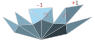
\includegraphics[scale=0.92]{svg/giftWrapping} \end{center}
\end{frame}


\section{Divide \& Conquer}

\begin{frame}{Слияние двух выпуклых оболочек}
	При слиянии необходимо вычислить цилиндр, состоящий из \\
	граней, соединяющих выпуклые оболочки \(\CH_1\) и \(\CH_2\).
\begin{center} 
\includegraphics[scale=1.04]{svg/CHconquer} \end{center}
\end{frame}


\begin{frame}{Поиск первой грани}
	Рассмотрим нижнюю вершину и её соседа в \(\CH_1\) \\
	и нижнюю вершину в \(\CH_2\). Проведём через них плоскость.

	Если кто-то из соседей выбранных вершин лежит ниже \\
	этой плоскости, заменим одну из вершин на него.

	Повторим процесс.\hspace{2.5cm}
	{\footnotesize \textcolor{white!46!dgray}{Картинка на доске}}
\end{frame}


\begin{frame}{Вычисление цилиндра}
	Заметим, что рёбра, ограничивающие цилиндр, являются \\
	рёбрами выпуклых оболочек \(\CH_1\) и \(\CH_2\).
\begin{center} 
\includegraphics[scale=1.04]{svg/CHconquerPolygonal} \end{center}
\end{frame}


\begin{frame}{Cylinder wrapping}
	Пусть \(p^1_i\) и \(p^2_j\)~— последние вершины, добавленные \\
	к цилиндру из \(\CH_1\) и \(\CH_2\) соответственно; \\
	\(p^1_i p^2_j p^*_k\)~— последняя известная грань цилиндра.

	Рассмотрим всех соседей \(p^1_i\) и \(p^2_j\) в их выпуклых оболочках, \\
	добавим грань \(p^*_* p^2_j p^1_i\), которая образует наибольший \\
	угол с \(p^1_i p^2_j p^*_k\), в цилиндр.

	Повторим, пока не придём к изначальному ребру.
\end{frame}


\begin{frame}{Время работы}
	Может показаться, что «проверяем всех соседей»~— долго.

	Однако заметим, что каждое ребро проверялось максимум \\
	дважды~— при поиске как первой грани, так и \\
	каждой из последующих.

	Отсюда сложность слияния линейна.

	\(T(n) = 2 T\lr*{\frac{n}{2}} + O(n)\) даёт время \(O\lr*{n \cdot \log n}\).
\end{frame}


\section{Lifting}

\begin{frame}{Сведéние {\it DT} к {\it 3D-\CH}}
	Покажем, что задача построения триангуляции Делоне \\
	на плоскости сводится к задаче построения выпуклой \\
	оболочки в \(\br^3\) за линейное время.

	Рассмотрим точки \(\{p_1, \ldots, p_n\} = S\) и поднимем их на параболоид:
	\[(x,y)\ \ \mapsto\ \ (x,y,x^2+y^2).\] \smallskip

\begin{thm}
	Проекции граней выпуклой оболочки, нормаль которых \\
	направлена вниз, будут областями Делоне.
\end{thm}
\end{frame}


\begin{frame}{Пересечения с плоскостями и окружности}
\begin{lm}
	Проекция пересечения параболоида \(z = x^2 + y^2\) и плоскости \\
	\(ax+by+cz=d\) на плоскость \(Oxy\)~— окружность. \\
	Её центр не зависит от \(d\).
\end{lm} \medskip

	{\bf Доказательство:} раскроем скобки, коэффициенты \\
	при \(x^2\) и при \(y^2\) будут одинаковы; выделенные полные \\
	квадраты не будут меняться при изменении \(d\).
\end{frame}


\begin{frame}{Почему это работает}
	Вершина выпуклой оболочки \(\CH(S)\)~— это первая точка \\
	касания \(S\) и какой-то плоскости, придвигаемой снаружи.
\begin{center} 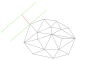
\includegraphics[scale=0.85]{svg/firstTangent} \end{center}
\end{frame}


\begin{frame}{Ещё о касании}
	Если касание произошло сразу в трёх точках~— значит, \\
	плоскость была параллельна грани выпуклой оболочки.

	Будем поднимать плоскость, параллельную грани \(\CH\), \\
	и одновременно смотреть, что происходит \\
	на плоскости \(Oxy\).
\end{frame}


\begin{frame}{Подъём плоскости}
\begin{center} 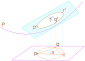
\includegraphics[scale=1.1]{svg/paraboloid} \end{center}
\end{frame}


\begin{frame}{Подъём плоскости — обоснование}
\begin{itemize}
	\item Рассмотрим плоскость, которая касается \(P\) в точке \(s^\prime\)~— \\
	поднятом центре описанной окружности. \medskip

	\item Начнём поднимать её вверх. Коэффициент \(d\) растёт. \\
	Проекция пересечения с \(P\)~— окружность с центром в \(s\). \\
	Радиус увеличивается. \medskip

	\item Первые точки на \(P\), которых коснётся плоскость, \\
	соответствуют первым точкам на \(Oxy\), через которые \\
	пройдёт расширяющаяся окружность. \medskip

	\item Треугольники Делоне соответствуют граням \CH.
\end{itemize}
\end{frame}


\begin{frame}{Диаграмма Вороного за \(n \cdot \log n\)}
\begin{itemize}
	\item Поднять точки на параболоид, \medskip
	\item Построить выпуклую оболочку, \medskip
	\item Спроецировать, получить триангуляцию Делоне, \medskip
	\item Перейти к двойственному графу, profit.
\end{itemize}
\end{frame}


\section{Двойственность точек и прямых}

\dualFrame{Определение}{
   \dualPoint{1}{1}{1} \dualPoint{-1.5}{-2}{2}
   \dualLinia{0.5}{0.5}{1} \dualLinia{0.25}{-1}{2}
}{\( (a,b)\ \ \longleftrightarrow\ \ \{y=ax-b\} \)}


\dualFrame{Инцидентность и над / под}{
   \dualPoint{1}{1}{1} \dualPoint{-1.5}{-2}{2}
   \dualLinia{0.5}{0.5}{1} \dualLinia{0.25}{-1}{2}
}{\(p \in l\ \ \Longleftrightarrow\ \ l^* \in p^*\)\hspace{2.5cm}
  \(p\) над \(l\)\ \ \(\Longleftrightarrow\)\ \ \(l^*\) над \(p^*\)}


\dualFrame{Ещё пример}{
   \dualPoint{-2}{1.5}{1} \dualPoint{1}{1.25}{2}
   \dualPoint{0}{-1.5}{3} \dualPoint{1}{-1.5}{4}
   \dualLinia{0.25}{2}{1} \dualLinia{-1.5}{-1.5}{2}
   \dualLinia{-0.5}{-0.5}{3} \dualLinia{1}{-3}{4}
   \draw[Plum](-2.2,2.5) node{{\footnotesize \(l_2\)}};
   \begin{scope}[xshift=8.5cm]
      \draw[HotPink] (-1.5,2.5) node {{\footnotesize \(p^*_1\)}}
                        (-2.5,-1.5) node {{\footnotesize \(p^*_4\)}};
   \end{scope}
}{\(l_1 \cap l_2 = p\ \ \Longleftrightarrow\ \ p^*\text{ проходит через }l_1^*,l_2^*\)}


\dualFrame{Двойственность задач}{
   \begin{scope}[xshift=8.5cm]
	\draw[thick,HotPink] (-4/3,-1.25) -- (-1,-1) -- (-1/6,0) -- (1.25,2.25);
   \end{scope}
	\dualLinia{-4 / 3}{1.25}{1} \dualLinia{-1}{1}{2}
	\dualLinia{-1 / 6}{0}{3} \dualLinia{5 / 4}{-2.25}{4}
	\dualLinia{0.5}{-1.5}{5} \dualLinia{-2 / 3}{-1.25}{6}
}{Верхнее пересечение полуплоскостей\ \ \(\Longleftrightarrow\)\ \ Нижняя \CH}


\begin{frame}{Спасибо за внимание!}
	\tableofcontents
\end{frame}

\end{document}
